\documentclass[]{article}
\usepackage{lmodern}
\usepackage{amssymb,amsmath}
\usepackage{ifxetex,ifluatex}
\usepackage{fixltx2e} % provides \textsubscript
\ifnum 0\ifxetex 1\fi\ifluatex 1\fi=0 % if pdftex
  \usepackage[T1]{fontenc}
  \usepackage[utf8]{inputenc}
\else % if luatex or xelatex
  \ifxetex
    \usepackage{mathspec}
  \else
    \usepackage{fontspec}
  \fi
  \defaultfontfeatures{Ligatures=TeX,Scale=MatchLowercase}
\fi
% use upquote if available, for straight quotes in verbatim environments
\IfFileExists{upquote.sty}{\usepackage{upquote}}{}
% use microtype if available
\IfFileExists{microtype.sty}{%
\usepackage{microtype}
\UseMicrotypeSet[protrusion]{basicmath} % disable protrusion for tt fonts
}{}
\usepackage[margin=1in]{geometry}
\usepackage{hyperref}
\hypersetup{unicode=true,
            pdftitle={R Assignment 3},
            pdfauthor={Chen Ming},
            pdfborder={0 0 0},
            breaklinks=true}
\urlstyle{same}  % don't use monospace font for urls
\usepackage{graphicx,grffile}
\makeatletter
\def\maxwidth{\ifdim\Gin@nat@width>\linewidth\linewidth\else\Gin@nat@width\fi}
\def\maxheight{\ifdim\Gin@nat@height>\textheight\textheight\else\Gin@nat@height\fi}
\makeatother
% Scale images if necessary, so that they will not overflow the page
% margins by default, and it is still possible to overwrite the defaults
% using explicit options in \includegraphics[width, height, ...]{}
\setkeys{Gin}{width=\maxwidth,height=\maxheight,keepaspectratio}
\IfFileExists{parskip.sty}{%
\usepackage{parskip}
}{% else
\setlength{\parindent}{0pt}
\setlength{\parskip}{6pt plus 2pt minus 1pt}
}
\setlength{\emergencystretch}{3em}  % prevent overfull lines
\providecommand{\tightlist}{%
  \setlength{\itemsep}{0pt}\setlength{\parskip}{0pt}}
\setcounter{secnumdepth}{0}
% Redefines (sub)paragraphs to behave more like sections
\ifx\paragraph\undefined\else
\let\oldparagraph\paragraph
\renewcommand{\paragraph}[1]{\oldparagraph{#1}\mbox{}}
\fi
\ifx\subparagraph\undefined\else
\let\oldsubparagraph\subparagraph
\renewcommand{\subparagraph}[1]{\oldsubparagraph{#1}\mbox{}}
\fi

%%% Use protect on footnotes to avoid problems with footnotes in titles
\let\rmarkdownfootnote\footnote%
\def\footnote{\protect\rmarkdownfootnote}

%%% Change title format to be more compact
\usepackage{titling}

% Create subtitle command for use in maketitle
\providecommand{\subtitle}[1]{
  \posttitle{
    \begin{center}\large#1\end{center}
    }
}

\setlength{\droptitle}{-2em}

  \title{R Assignment 3}
    \pretitle{\vspace{\droptitle}\centering\huge}
  \posttitle{\par}
    \author{Chen Ming}
    \preauthor{\centering\large\emph}
  \postauthor{\par}
      \predate{\centering\large\emph}
  \postdate{\par}
    \date{May 20th}


\begin{document}
\maketitle

\hypertarget{section}{%
\paragraph{2017022002}\label{section}}

\hypertarget{part-1}{%
\section{Part 1}\label{part-1}}

\hypertarget{find-descriptive-statistics-of-the-data-and-summarize-them-into-a-table}{%
\paragraph{\texorpdfstring{\textbf{1.1. Find descriptive statistics of
the data and summarize them into a
table}}{1.1. Find descriptive statistics of the data and summarize them into a table}}\label{find-descriptive-statistics-of-the-data-and-summarize-them-into-a-table}}

Experiment details are omitted here.

\hypertarget{use-graphical-analysis-to-investigate-the-relationship-between-alumni-giving-rate-and-each-of-the-other-variables}{%
\paragraph{\texorpdfstring{\textbf{1.2. Use graphical analysis to
investigate the relationship between Alumni Giving Rate and each of the
other
variables}}{1.2. Use graphical analysis to investigate the relationship between Alumni Giving Rate and each of the other variables}}\label{use-graphical-analysis-to-investigate-the-relationship-between-alumni-giving-rate-and-each-of-the-other-variables}}

Scatter plot is demonstrated as follows. In the first and the third
graphs, we can find that points cluster closely around fitted lines.
While in the second graph, points seem to drift away from fitted line.
From the graphical analysis, we can reasonably assume that alumni giving
rate is more closely related to both graduation rate and faculty rate
than number of classes under 20.
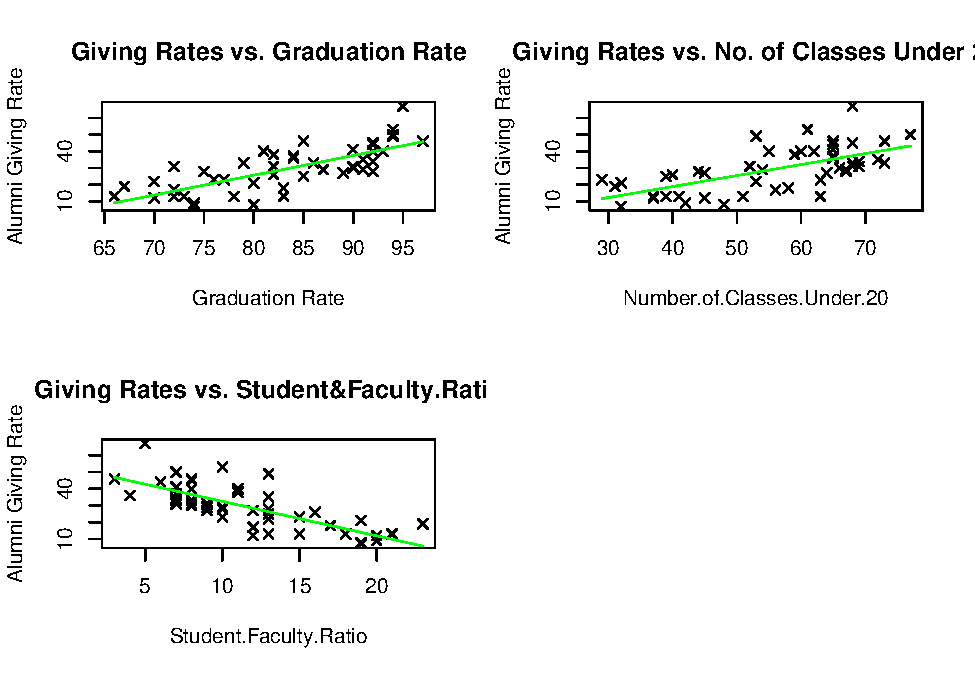
\includegraphics{Assign3_Rmarkdown备份_files/figure-latex/unnamed-chunk-1-1.pdf}

\hypertarget{develop-a-multiple-linear-regression-model-that-could-be-used-to-predict-the-alumni-giving-rate-using-the-data-provided}{%
\paragraph{\texorpdfstring{\textbf{1.3.Develop a multiple linear
regression model that could be used to predict the Alumni Giving Rate
using the data
provided}}{1.3.Develop a multiple linear regression model that could be used to predict the Alumni Giving Rate using the data provided}}\label{develop-a-multiple-linear-regression-model-that-could-be-used-to-predict-the-alumni-giving-rate-using-the-data-provided}}

We can use \textbf{stepAIC} method to construct the best multi-linear
regression model from a set of candidate variables.The experiment result
indicates that, AIC value becomes smaller when the variable
\textbf{``Number of classes under 20''} is deleted from the regression
model. The lowest AIC value is \textbf{196.7}. Since smaller AIC value
means better fitting effect, we should construct a regression model with
\textbf{``Graduation Rates''} and \textbf{``Student \& Faculty Ratios''}
as independent variables. The linear regression model fomula is
constructed as \[y=-19.1063+0.7557x_{1}-1.2460x_{2}\]where \(y\) denotes
alumni giving rate, \(x_{1}\) denotes graduation rate, \(x_{2}\) denotes
student\&faculty ratio.

\hypertarget{check-the-model-assumptions}{%
\paragraph{\texorpdfstring{\textbf{1.4.Check the model
assumptions}}{1.4.Check the model assumptions}}\label{check-the-model-assumptions}}

In Q-Q graph, points closely cluster around the line, which proves that
the assumption of \textbf{normality} is satisfied; there is no reason to
assume that graduation ratio and faculty to student ratio is related.
Therefore, the assumption of \textbf{independence} is satisfied;from
graph one, we can observe that residuals has no systematic relationship
between residuals and the predicted values. The model well captures
systematic variance in the data, thereby proves that the assumption of
\textbf{Linearity} is satisfied; the Scale-Location graph shows that the
points form a random band around the horizontal line. Hence the
assumption of \textbf{Homoscedasticity} is satisfied.
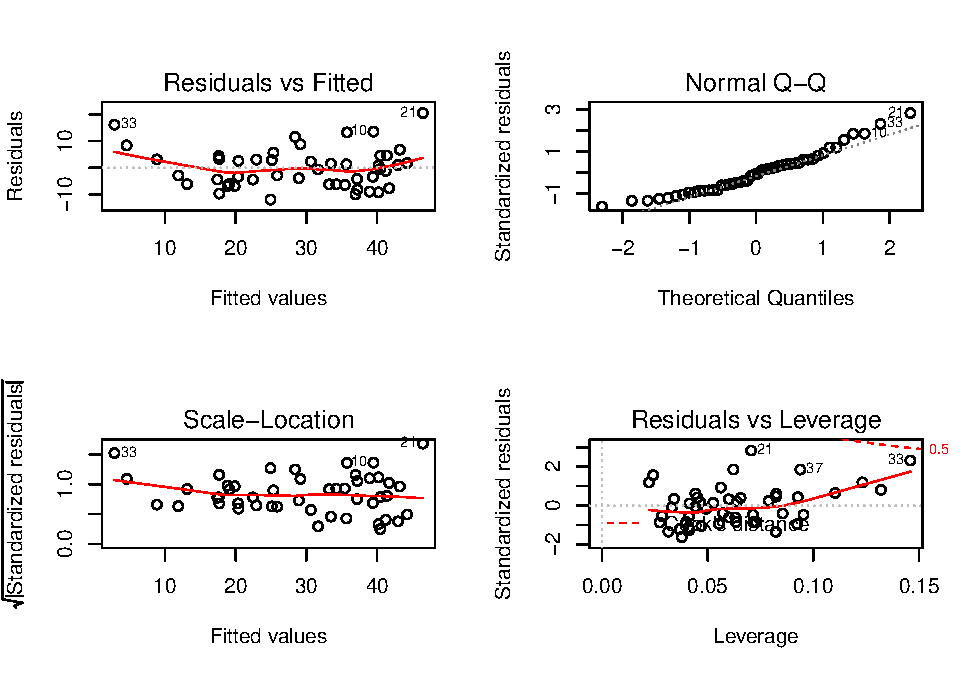
\includegraphics{Assign3_Rmarkdown备份_files/figure-latex/unnamed-chunk-3-1.pdf}

\hypertarget{part-2}{%
\section{Part 2}\label{part-2}}

\hypertarget{calculate-the-mean-of-fertility-and-partition-the-provinces-into-two-groups}{%
\paragraph{\texorpdfstring{\textbf{2.1. Calculate the mean of Fertility
and partition the provinces into two
groups}}{2.1. Calculate the mean of Fertility and partition the provinces into two groups}}\label{calculate-the-mean-of-fertility-and-partition-the-provinces-into-two-groups}}

The mean of fertility in stated provinces is \textbf{70.14255}.
Experiment details are omitted here.

\hypertarget{use-logistic-regression-to-show-the-relationship-between-y-and-the-other-variables-and-then-interpret-the-regression-results}{%
\paragraph{\texorpdfstring{\textbf{2.2. Use logistic regression to show
the relationship between y and the other variables and then interpret
the regression
results}}{2.2. Use logistic regression to show the relationship between y and the other variables and then interpret the regression results}}\label{use-logistic-regression-to-show-the-relationship-between-y-and-the-other-variables-and-then-interpret-the-regression-results}}

The experiment result shows that \textbf{Agricluture},
\textbf{Examination} and \textbf{Education} are negatively related to
Fertility, with remaining factors positively related to Fertility.
P-values for \textbf{Examination} and \textbf{Agriculture} are 0.0203
and 0.0165 respectively. While p-values for other factors are all beyond
the range of significance. The experiment result indicates that
fertility in selected provinces is significantly related to
\textbf{Agriculture} and \textbf{Examination} under significance level
of 0.05. It implies that fetility is closely related to agriculture
situation and examination circumstance in the provinces.

\hypertarget{choose-a-model-selection-criterion-for-instances-aic-bic-adjusted-r-square-or-cp-and-use-it-to-select-a-reasonable-model}{%
\paragraph{\texorpdfstring{\textbf{2.3. Choose a model selection
criterion, for instances, AIC, BIC, adjusted R square or Cp, and use it
to select a reasonable
model}}{2.3. Choose a model selection criterion, for instances, AIC, BIC, adjusted R square or Cp, and use it to select a reasonable model}}\label{choose-a-model-selection-criterion-for-instances-aic-bic-adjusted-r-square-or-cp-and-use-it-to-select-a-reasonable-model}}

We can construct the best multi-linear regression model from a set of
candidate variables. Under AIC criterion, regression model with smaller
AIC value is considered better. The experiment result indicates that AIC
value gets smallest(at -85.27) when the variables ``Catholic'' and
``Education'' are deleted from the regression model. Hence we should
construct a regression model with \textbf{``Infant.Mortality''},
\textbf{``Agriculture''} and \textbf{``Examination''} as independent
variables. The regression model constructed is: \begin{equation}
y = 1.05056-0.00811x_{1}-0.05017x_{2}+0.03501x_{3}
\end{equation} where \(x_{1}\), \(x_{2}\), and \(x_{3}\) denotes
\textbf{Agriculture}, \textbf{Examination}, and \textbf{Infant
Mortality} respectively.


\end{document}
